\documentclass[11pt]{article}
\usepackage[utf8]{inputenc}

\usepackage[margin=2.1cm]{geometry}
\usepackage[utf8]{inputenc}
\usepackage{dirtytalk}
\usepackage{titling} % multiple title pages

% \usepackage{bookmark}% http://ctan.org/pkg/bookmark

\usepackage{pdfpages}
\usepackage{soul}
\pdfminorversion=7

\usepackage{xurl}


\title{}
% \author{Ryan-Rhys Griffiths}
\date{}

\makeatletter
\renewcommand\@bibitem[1]{\item\if@filesw \immediate\write\@auxout
    {\string\bibcite{#1}{Exhibit \the\value{\@listctr}}}\fi\ignorespaces}% <------------
\def\@biblabel#1{Exhibit #1:}% <-------------------
\makeatother


\usepackage{amsmath}
\usepackage{amssymb}
\usepackage[labelfont=bf]{caption}
\usepackage{setspace}\setstretch{1.167} % prerequisite of geometry
\usepackage[utf8]{inputenc}
\usepackage[british, cleanlook]{isodate}
\usepackage[pagewise, modulo, displaymath, mathlines]{lineno}
\usepackage{microtype}
\usepackage[amssymb]{SIunits}
\usepackage[bib, enum, eqno, lineno, toc]{tabfigures}

\usepackage{fancyhdr}
\usepackage{soul}
\usepackage{tikz}
\setlength\parindent{0pt}
\newcommand{\mybullet}{\,\textbullet\,}

\setcounter{tocdepth}{4}
\setcounter{secnumdepth}{4}


\pagestyle{fancy}
\fancyhf{}
%\tikz[remember picture, overlay] \node at (current page.center) {\includegraphics{outline_letterhead}};
\renewcommand{\headrulewidth}{1pt}
% \cfoot{\vspace{-5em}\textbf{\so{\MakeUppercase{Razvan V. Marinescu}}}\\\smallskip\footnotesize Postdoctoral Associate in Artificial Intelligence for Healthcare\\ 

\lhead{EB-1A Permanent Residence Petition for Dr. Ryan-Rhys Griffiths}
% toggle for I-485
% \lhead{I-485 Application to Register Permanent Residence or Adjust Status for Dr. Ryan-Rhys Griffiths}
% \rhead{\thepage}
\cfoot{\thepage}

\begin{document}
\newcommand{\tc}[1]{\textcolor{blue}{#1}}

\tc{Attach checks with clipper. Always check the USCIS website for the most recent fees! See check writing instructions: https://www.uscis.gov/forms/filing-fees}

\begin{figure}
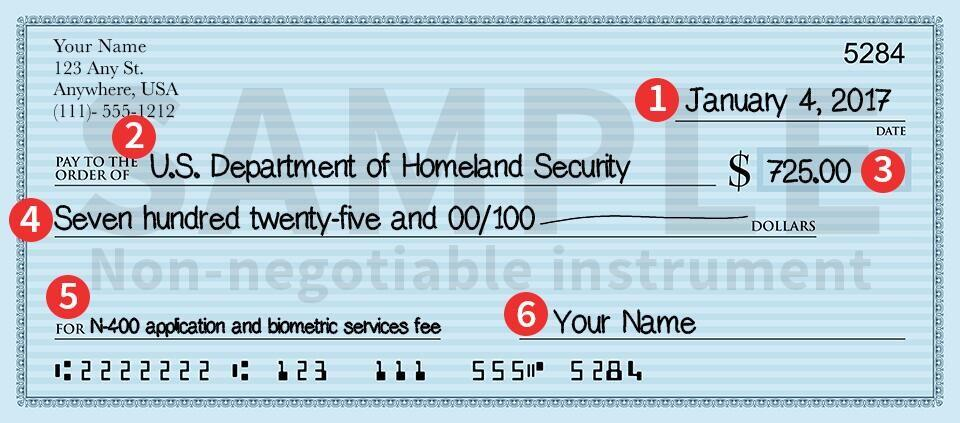
\includegraphics[width=0.8\textwidth]{aux/check.jpeg}
\end{figure}

\vspace*{5em}

\begin{center}
\Large{\textbf{TABLE OF CONTENTS}} 
\end{center}

\begin{enumerate}
 \item Form G-1145 e-Notification of Application/Petition Acceptance
 \item Form I-140, Immigrant Petition for Alien Worker, with \$700 filing fee
 \item Form I-907, Request for Premium Processing Service, with the \$2,500 filing fee
 \item Photocopies of the passport, J-1 visa stamp, DS-2019, Form I-797 and most recent Form I-94 for the O1A visa
 \item Initial Evidence in Support of the I-140 Immigrant Petition
 \item Statement from Dr. Ryan-Rhys Griffiths detailing plans on how he intends to continue work in the United States
 \item List of Exhibits
 \item Exhibits 1--44
\end{enumerate}

% TOC for I-485

% \begin{enumerate}
%  \item Form G-1145 e-Notification of Application/Petition Acceptance
%  \item Form I-485, Application to Register Permanent Residence or Adjust Status, with \$1225 filing fee + biometrics services
%  \item Form I-765 Application for Employment Authorization
%  \item Form I-693 Report of Immigration Medical Examination and Vaccination Record (Sealed Envelope)
%  \item Photocopies of the passport, J-1 visa stamp, DS-2019, Forms I-797 and Forms I-94 for the J1 and the O1A visa, Form I-797 receipt and approval notices for the approved I-140 petition
%  \item Signed statement from Dr. Ryan-Rhys Griffiths detailing plans on how he intends to continue work in the United States
%  \item Copy of birth certificate
%  \item 2x passport photos for Form I-765
%  \item 2x passport photos for Form I-485
% \end{enumerate}


\pagebreak
\sloppy
\vspace{4em}

\begin{center}
 \Large{\textbf{Initial Evidence in Support of the I-140 Immigrant Petition}}
\end{center}

\vspace{4em}

\begin{tabular}{ll}
\textbf{Petitioner and Beneficiary:} & Ryan-Rhys Griffiths\\
\textbf{Classification Sought:} & Employment-Based Immigration, First Preference\\
& Extraordinary Ability in Science (EB-1A).\\
& Sec. 203(b)(1) INA [8 U.S.C. 1153].\\
\end{tabular}

\vspace{2em}

To whom it may concern,

\vspace{2em}

\newcommand{\fie}{Machine Learning and the Natural Sciences}
\newcommand{\dr}{Dr. Griffiths }
\newcommand{\drs}{Dr. Griffiths's }

\newcommand{\qu}[1]{\say{\emph{#1}}}

\newcommand{\dg}{(Prof. XYZ, Professor of XYZ, University of XYZ)\\}
\newcommand{\bc}{(Prof. XYZ, Professor of XYZ, University of XYZ)\\}
\newcommand{\pl}{(Prof. XYZ, Professor of XYZ, University of XYZ)\\}
\newcommand{\bw}{(Prof. XYZ, Professor of XYZ, University of XYZ)\\\\}
\newcommand{\sk}{Prof. XYZ, Professor of XYZ, University of XYZ)\\}
\newcommand{\ag}{Prof. XYZ, Professor of XYZ, University of XYZ)\\}

This letter is respectfully submitted in support of the petition of Dr. Ryan-Rhys Griffiths for classification as a qualified immigrant under the first preference employment immigration for Aliens of Extraordinary Ability pursuant to section 203(b)(1)(A) of the Immigration and Nationality Act (“the Act”). This evidence shows that Dr. Griffiths is an alien of extraordinary ability in the sciences, specifically in \underline{\fie{}}, who has sustained national and international acclaim with his achievements recognized in the field of expertise. More precisely, this letter provides evidence that:
\begin{enumerate}
 \item \dr satisfies \underline{four} of ten criteria listed in 8
CFR, Section 204.5(h)(3), namely:
\begin{itemize}
 \item \dr has made original scientific and scholarly contributions of major significance in the field of \fie{}. (section \ref{original})
 \item \drs authorship of scholarly articles in the field in professional or major trade publications or other major media. (section \ref{authorship})
 \item Participation of \dr as a judge of the work of others in the field (section \ref{reviews})
\item Published material about \dr in professional or major trade publications or other major media, relating to \drs work in the field (section \ref{media})
\end{itemize}
 \item \dr reached a level of expertise indicating that he is one of that small percentage who have risen to the very top of the field of \fie{} -- section \ref{risentotop}.
 \item \dr sustained national or international acclaim and that his achievements have been recognized in the field of \fie{} -- section \ref{sustanedacclaim}.
\end{enumerate}


Pursuant to 8 CFR, Section 204.5(h)(1), \dr may file an I-140 visa petition for classification under Section 203(b)(1)(A) of the Act as an alien of extraordinary ability in the sciences on his own behalf.\\

Pursuant to 8 CFR, Section 204.5(h)(5), neither an offer for employment in the United States nor a labor certification is required for this classification.


\newpage
\section{Summary of \drs achievements and qualifications}

\dr is a Postdoctoral Research Scientist in the Adaptive Experimentation team at Meta Research, Menlo Park, California \cite{metaoffer}. \dr joined Meta Research in August 2022 after completing his PhD from the University of Cambridge in the United Kingdom (UK). His research focusses on \fie{}. Before coming to the US, \dr lived in the UK for 10 years, completing his undergraduate studies at Imperial College London, and his masters and PhD degrees at the University of Cambridge, two leading universities worldwide \cite{cv} \cite{degrees}. \dr graduated with First Class Honours in Chemistry with Molecular Physics from Imperial College London \cite{degrees}.\\



\dr works on machine learning methodologies, namely Gaussian processes and Bayesian optimization as well as applications of machine learning in the natural sciences. Bayesian optimization is currently utilized across many areas of artificial intelligence (AI) as a state-of-the-art hyperparameter optimizer for machine learning algorithms making the deployment of AI solutions both cheaper and faster. Bayesian optimization is also a core methodology for accelerating the discovery of novel materials and molecules in areas such as drug discovery and renewable energy. \dr has worked for over 6 years on improving Bayesian optimization methodology to achieve speedups and cost-savings for AI algorithms as well as for the discovery of novel molecular and chemical materials. \\


\dr has made major contributions to the field of machine learning and the natural sciences. He was the lead author on one of the first papers to leverage generative AI for drug molecule generation, a field which promises to accelerate the discovery of therapeutics for conditions including cancer, Parkinson’s disease, and diabetes (section \ref{conbo}). He has also coauthored Heteroscedastic Evolutionary Bayesian Optimisation (HEBO), a state-of-the-art machine learning algorithm that won the 2020 NeurIPS Black-box optimization challenge, a competition sponsored by Meta and Twitter at NeurIPS, the world’s premier machine learning conference. HEBO has subsequently been used by the ATLAS experiment group at the Large Hadron Collider in CERN (section \ref{hebo}). \dr has also leveraged machine learning directly to discover novel photoswitch molecules, a class of compound with applications as agents for vision restoration in the blind, as anti-cancer therapeutics, as well as for environmental applications in renewable energy (section \ref{photoswitch}). More recently, \dr has coauthored a paper which analyzes the mathematical capabilities of ChatGPT that has acquired 194 citations this year alone (section \ref{chatgpt}). \\

To date, \dr has published over 20 peer-reviewed scientific articles (7 as lead author) that have been featured in top journals in the machine learning and science fields. The articles \dr authored have accrued 1042 citations as of November 2023 and have been cited more than 500 times in the past 11 months, showing a marked increase in the impact of his research. Additionally, \drs papers have accrued significantly more citations than the articles of his peers (section \ref{articlespeers}). \\


\dr has been active as a judge of the work of others having conducted 49 peer reviews in 23 leading journals in the field of \fie{} (section \ref{reviews}). \\


\drs research has received significant media attention. He maintains 18,000+ followers on LinkedIn and 4,000+ followers on Twitter. His paper on the mathematical capabilities of ChatGPT was featured in Synced, a leading online AI technology and industry review outlet (section \ref{synced}). His GAUCHE and FlowMO software libraries have been used in industry by the AstraZeneca AI group and Relay Therapeutics, an American biotechnology company. (section \ref{relay}). \\


As evidenced by six recommendation letters from distinguished professors and managers in the machine learning industry, his 20+ scientific publications, 49 peer-reviews, \dr has risen to the top of the field of \fie{} (section \ref{risentotop}). \dr has further sustained this performance as evidenced by the increasing number of citations he has recently obtained (500+ in the past 11 months alone).


\section{Proof of \drs Extraordinary Ability}

\subsection{Evidence of original scientific, scholarly, artistic, athletic, or business-related contributions of major significance to the field}
\label{original}

\subsubsection{Evidence of original scientific contribution: One of the first papers using generative AI to propose novel drug molecules}
\label{conbo}

\dr introduced one of the first algorithms to apply generative AI, namely variational autoencoders, to the targeted generation of novel drug molecules which will accelerate the adoption of new and effective medical treatments. At the time of publishing in 2017, Dr. Griffiths’s algorithm represented the state-of-the-art in machine-learning based molecule generation. While in 2023, it is no longer the state-of-the-art algorithm, it has catalyzed advances in molecule generation methods as evidenced by 334 citations following its publication in the Chemical Science journal, the flagship journal of the Royal Society of Chemistry \cite{gscholar, conbo}. \\

\qu{% ACD 
To provide more specifics on the details of \drs research, I will begin by discussing his work on “Constrained Bayesian Optimization for Automatic Chemical Design using Variational Autoencoders”. In this work Dr. Griffiths improved a system for extending Bayesian optimization to high-dimensional and structured input spaces by using a variational autoencoder (VAE), a deep learning methodology that facilitates transformation of discrete variables such as graphs, strings, and bit vectors to a continuous latent representation. \drs methodological contribution in this paper was to first highlight a problem in existing VAE- based Bayesian optimization architectures, namely the mismatch between the objectives of the Bayesian optimization Gaussian processes surrogate and the training set support of the VAE. The crux of this problem is that there is a tendency for the Bayesian optimization scheme to select points that lie far away from the support of the VAE training distribution yielding invalid outputs. In his paper, \dr implemented a constraint scheme which increased the number of valid outputs from the model, yielding state-of-the-art performance at the time of its introduction.} \\\\\sk


\qu{\dr has provided many core research contributions within the field of Bayesian optimization. With his paper, "Constrained Bayesian optimization for Automatic Chemical Design using Variational Autoencoders", published in Chemical Science, Griffiths improved on the incumbent state-of-the-art in machine learning-based molecular property optimization. This paper also represented a fundamental advance in Bayesian optimization methodology. Scaling Bayesian optimization to high-dimensional problems has traditionally been a challenging research problem. In his paper, \dr successfully applies variational autoencoders as a tool to reduce the dimensionality of the optimization space facilitating efficient search for novel molecules. \drs core contribution in this regard was to implement a probabilistic constraint scheme that addressed the problem of invalid generation from the latent space of the variational autoencoder yielding significant performance gains compared to previous algorithms. To date, Dr. Griffiths has received over 260 citations for this contribution alone.} \\\\ \ag

% HEBO 
\subsubsection{Evidence of original scientific contribution: Coauthored HEBO, the winning algorithm in the 2020 NeurIPS black-box optimization competition}
\label{hebo}

\dr coauthored the Heteroscedastic Evolutionary Bayesian Optimization (HEBO) algorithm which achieved 1st place at the 2020 NeurIPS black-box optimization competition sponsored by Twitter and Meta, a competition organized at the world's premier machine learning conference. The algorithm was awarded a \$6,000 prize for winning the challenge (https://bbochallenge.com/leaderboard/). To this day, HEBO remains a state-of-the-art algorithm for machine learning hyperparameter tuning and has been used earlier this year by the ATLAS experiment at the Large Hadron Collider in CERN (section~\ref{citations}). It is heavily used in research and industry as evidenced by 1,900+ stars on GitHub (\url{https://github.com/huawei-noah/HEBO}) as well as 115 citations as of November 2023. It was published in the prestigious Journal of Artificial Intelligence Research in 2022. \cite{hebo}. The algorithm has subsequently been used as a benchmark algorithm for machine learning-based antibody design against the SARS-CoV (COVID) antigen:

\begin{itemize}
    \item Khan, A., Cowen-Rivers, A.I., Grosnit, A., Robert, P.A., Greiff, V., Smorodina, E., Rawat, P., Akbar, R., Dreczkowski, K., Tutunov, R. and Bou-Ammar, D., Toward real-world automated antibody design with combinatorial Bayesian optimization. Cell Reports Methods, p.100374, 2023.
\end{itemize}

and as a hyperparameter optimization algorithm for robotics amongst other applications:

\begin{itemize}
    \item Liu, P., Tateo, D., Bou-Ammar, H. and Peters, J., Efficient and reactive planning for high speed robot air hockey. In 2021 IEEE/RSJ International Conference on Intelligent Robots and Systems (IROS) (pp. 586-593). 2021.
\end{itemize}

Further details on the HEBO algorithm are provided by Dr. XYZ and Prof. XYZ:\\\\


\qu{% HEBO
Ryan-Rhys Griffiths’s second work is related to the Heteroscedastic Evolutionary Bayesian Optimization (HEBO) algorithm. This algorithm won the 2020 NeurIPS Black- Box Optimization Competition. The NeurIPS conference is the top international venue for machine learning research. The HEBO algorithm currently has 115 citations and has been published in the prestigious Journal of Artificial Intelligence Research. The algorithm showed the strongest performance on machine learning hyperparameter tuning tasks in the competition by introducing novel methods for considering heteroscedasticity and non-stationarity of the underlying data via input warping using a Beta Kumaraswamy distribution function and Yeo-Johnson and Box-Cox transforms to correct for heteroscedasticity.} \\\\\bw 

\qu{\dr has gone on to achieve notable international success in his research. For instance, he jointly developed the heteroscedastic evolutionary Bayesian optimisation (HEBO) algorithm that won the 2020 NeurIPS Competition on Black-Box Optimisation. The HEBO algorithm has subsequently been used notably in the ATLAS experiments at the Large Hadron Collider at CERN.} \\\\ \dg


% Gaussian processes for molecules
\subsubsection{Evidence of original scientific contribution: Lead author on a series of papers using Gaussian processes to discover novel photoswitch molecules}
\label{photoswitch}

\dr was lead author on the paper, “Data-driven discovery of molecular photoswitches using multi output Gaussian processes. In this work, \dr used a machine learning algorithm based on multioutput Gaussian processes with a Tanimoto kernel to identify a promising photoswitch molecule. The paper was published in Chemical Science, the flagship journal of the Royal Society of Chemistry and was featured as one of the most popular physical and theoretical chemistry articles of 2022 \cite{most_pop}. The collection is described as follows, \say{This specially curated collection pulls together some of the most popular articles from 2022 in the field of physical and theoretical chemistry. The collection presents some outstanding contributions to the field, ranging from deep learning models for predicting drug-target interactions, through to investigations into colour-tunable persistent luminescence in low-dimensional zinc-organic halide microcrystals.} \cite{most_pop}. The paper has acquired 34 citations to date. \dr has additionally made his methodology freely available as the open-source FlowMO and GAUCHE libraries to be used by researchers in academia and in industry. His paper FlowMO was awarded a spotlight contributed talk at the 2020 NeurIPS workshop on machine learning for molecules i.e. it was ranked in the top 5\% of accepted papers: \url{https://neurips.cc/virtual/2020/protected/workshop_16136.html}. His FlowMO software library has subsequently been used by the AstraZeneca AI group (section~\ref{citations}) as well as Relay Therapeutics (section~\ref{relay}), a US biotechnology company \cite{media}. His GAUCHE software library was accepted at NeurIPS 2023 \cite{neurips_papers}, the world's premier international machine learning conference \cite{gscholar}: \url{https://neurips.cc/virtual/2023/poster/70081} \\

\qu{I first noticed \drs work in 2019 when working on Bayesian set optimization and discovering his excellent work around using the Tanimoto kernel in the context of molecular chemistry. Looking at his then already substantial track-record and impact, I also realized with amazement that he was still at an early stage of his career (then a PhD student at Cambridge) and upon our discussions online and in [insert placename] I was stunned by his rare computational intelligence and scientific versatility. I must also say that with two of my students we studied and reproduced some of his work, and despite our efforts to find a better approach we ended up corroborating his conclusions and further showing some advantages of the kernel he used in terms of the associated prediction uncertainty.} \\\\ \dg 

\qu{The contribution of GAUCHE is to make available the Gaussian process framework to operate on spaces of molecules, chemical reactions, and proteins. The library is the first to make available modern machine learning frameworks such as PyTorch and Tensorflow (and GPU-based computation) to Gaussian process-based molecular property prediction. The library has already received international attention from the machine learning community with a spotlight (top 5\% of accepted papers) at the 2020 NeurIPS Workshop on Machine Learning for Molecules for the paper “Molecular Property Prediction with FlowMO” and has even seen usage in the industry which is rare on such a short timeframe. } \\\\ \sk

\qu{\dr released a number of open-source software packages during his PhD, the most notable of which have been the GAUCHE and FlowMO libraries which are currently being used internationally for research in machine learning for chemistry and chemical reaction optimization, as well as in the pharmaceutical industry. The libraries combined have over 100 GitHub stars.} \\\\ \pl

\qu{The FlowMO paper was awarded a spotlight at the 2020 NeurIPS Workshop on Machine Learning for Molecules, a major international venue for discussions on machine learning applied to the molecular sciences. In detail, the FlowMO and GAUCHE software libraries extend Gaussian processes to operate on molecular representations. The particular focus of the work is on commonly-used representations for molecules such as SMILES strings, binary vectors, and graphs. The open-source software implementations are the first to support graphics processing unit (GPU) based machine learning on molecules using Gaussian processes in a modern machine learning framework. The aforementioned considerations are key to making these technologies available to practitioners. So far, in spite of its recency, \drs research has seen significant uptake in industry with users of GAUCHE including AstraZeneca and Relay Therapeutics.} \\\\ \bc


\subsubsection{Evidence of original scientific contribution: Coauthored a paper on the mathematical capabilities of ChatGPT.}
\label{chatgpt}

% ChatGPT

Dr. Griffiths coauthored a paper that critically analyzed the mathematical capabilities of ChatGPT. To date the paper has accrued 194 citations in the past year alone \cite{gscholar} and has attracted media attention, being featured in Synced, China’s leading machine learning periodical. \cite{media}. The paper has recently been accepted to NeurIPS 2023 \cite{neurips_papers}, the world's premier international machine learning conference \cite{gscholar}: \url{https://neurips.cc/virtual/2023/poster/73421} \\ 

\qu{\dr recently coauthored a paper analyzing the mathematical capabilities of ChatGPT. This paper concluded that ChatGPT did not possess the skills of a graduate level mathematician based on a series of tasks involving proof completion, symbolic integration, and performance assessment as a mathematical search engine. The paper has already received 6 citations in the past month and will serve an important purpose in highlighting some of the limitations of ChatGPT for prospective deployment in the education system.} \\\\ \sk


\subsection{Evidence of authorship of scholarly articles in professional or major trade publications or other major media}
\label{authorship}

\subsubsection{\dr has published 23 scientific articles in the field  of machine learning and the natural sciences}

As evidenced in \drs Curriculum Vitae \cite{cv} and in his Google Scholar profile \cite{gscholar}, Dr. Griffiths has so far authored 23 scientific articles (7 as lead author), which have together gathered 1042 citations \cite{gscholar} as of November 2023. \drs publications are presented in \cite{conbo} through \cite{msci}.


\subsubsection{\drs publications have been published in the leading journals and conferences in his field}

As preliminary definitions, the h5-index is the h-index for articles published in the last 5 complete years. It is the largest number h such that h articles published in 2018-2023 have at least h citations each. As a concrete example, if a journal has 100 publications published within the period 2018-2023 each having at least 100 citations or more, the journal's h5-index will be 100. The Impact Factor (IF) is a number quantifying the number of citations an article receives in the 2 years since its publication. an IF $> 10$ indicates that the journal belongs to the top 1.9\% journals worldwide and an IF $> 6$ indicates that the journal belongs to the top 5.41\% \cite{impact_factor}. \drs scientific articles have been published in the leading venues in \fie{}, which include:
\begin{itemize}
    \item Advances in Neural Information Processing (NeurIPS): h5-index: 309 and the 9th ranked publication venue across all areas of research indexed by Google Scholar (Exhibit 21). \dr has authored two articles in NeurIPS \cite{cv, gauche, chatgpt}
    \item The International Conference on Machine Learning (ICML): A top tier conference in machine learning research with a Google Scholar h5-index of 254 and the 17th ranked publication venue across all fields of research indexed by Google Scholar [Exhibit 21]. \dr authored one article on machine learning in ICML \cite{sensors}.
    \item The Journal of Artificial Intelligence Research (JAIR): A top journal in machine learning and artificial intelligence with an Impact Factor of 2.776. \dr authored one article on Bayesian optimization in JAIR \cite{cv, hebo}.
    \item The Journal of Machine Learning Research (JMLR): JMLR is the premier journal for machine learning research with a h5-index of 106 and an Impact Factor of 5.177. \dr authored one article on Bayesian optimization in JMLR \cite{cv, forget}.
    \item Accounts of Chemical Research: A top journal in chemistry [Exhibit 21] with a h5-index of 163, an Impact Factor of 18.3, and the 84th ranked publication venue across all fields of research indexed by Google Scholar [Exhibit 21]. \dr authored one paper on machine learning applications to chemistry in Accounts of Chemical Research \cite{cv, mapping}.    
    \item Chemical Science: The flagship journal for the Royal Society of Chemistry with a h5-index of 132 and an Impact Factor of 9.969. \dr has published two papers on machine learning applications in chemistry in Chemical Science \cite{cv, photo}.
    \item The Astrophysical Journal: A leading journal in astrophysics with a h5-index of 169, an Impact Factor of 5.874, and the 68th ranked publication venue across all fields of research indexed by Google Scholar [Exhibit 21]. \dr has published one paper on applications of Gaussian processes to high-energy astrophysics in the Astrophysical Journal \cite{cv, mrk}.
    \item Machine Learning: Science and Technology (MLST): A journal published by the Institute of Physics with an Impact Factor of 6.8. \dr has published one paper on Bayesian optimization in MLST \cite{cv, achieving}.
    \item Applied AI Letters: A new journal published by Wiley with an Impact Factor of 1.2. \dr has published one paper on machine learning in Applied AI Letters \cite{cv, bourached}
    \item Electronic Imaging: A leading conference in applications of computer vision. \dr has coauthored 4 papers on applications of AI to the fine arts in Electronic Imaging \cite{cv, raiders, greg, saints, res}.
\end{itemize}

Prof. XYZ, the examiner of \drs PhD thesis has verified that \drs work has been published in leading venues in the field.\\

\qu{Dr. Griffiths’s first author work was published in \underline{prestigious international journals in their respective fields}: The Astrophysical Journal (Impact Factor: 5.874), Chemical Science (Impact Factor: 9.969), and Machine Learning: Science and Technology (Impact Factor: 6.013). Dr. Griffiths was also a core contributor to several other papers during his PhD published in venues such as The International Conference on Machine Learning (h5-index: 237) and The Accounts of Chemical Research (Impact Factor: 24.47). }\\\\ \pl

\subsubsection{\drs scientific articles have been cited significantly more than the articles of his peers}
\label{articlespeers}

It is worth noting that in Kazarian v. USCIS, 596 F.3d 1115, 1121 (9th Cir. 2010) the court confirmed that the act of publication was sufficient, and rejected the Service’s view that petitioner must show other scholars have cited his work. Based on the aforementioned, the above-stated is sufficient evidence to meet the plain language of the criterion of evidence of authorship of scholarly articles in professional or major trade
publications or other major media. However, \drs work has also been cited extensively as will be described here. \\

The works authored by \dr have attained significantly more citations than the average for the field as gauged by the impact factor of the journals his work has been published in. \drs articles in Chemical Science have achieved 200+ citations and 34 citations respectively in the two years since their publication [Exhibit 1], significantly higher than the average of 9.969 for the impact factor. His paper in the Journal of Artificial Intelligence Research has attained 115 citations in under two years since its publication, significantly higher than the impact factor of 2.776. His paper in Accounts of Chemical Research has attained 50+ citations significantly more than the impact factor of 18.3. Dr. Griffiths’s paper in JMLR has received 15 citations, which is higher than the Impact Factor of 5.177. Lastly, Dr. Griffiths’s papers in MLST and the Astrophysical Journal have received 35 citations, and 17 citations respectively, also higher than the Impact Factors of 6.8 and 5.874. When taking all publications of \dr into account, his 1042 citations gathered so far place him within the top 1\% percentile of scholars in Computer Science according to the ESI ranking \cite{esi}.

\subsection{Evidence that \dr has been asked to judge the work of others in machine learning and the natural sciences}
\label{reviews}

\dr has been a reviewer for the top journals and conferences in machine learning and the sciences \cite{reviews}. \dr has reviewed a total of 49 scientific articles including:
\begin{itemize}
    \item Advances in Neural Information Processing (NeurIPS): h5-index: 309 and the 9th ranked publication venue across all areas of researched indexed by Google Scholar (Exhibit 21). \dr has reviewed 10 articles for this conference.
    \item Nature Machine Intelligence: With an Impact Factor of 23.8, Nature Machine Intelligence is a leading journal in machine learning and artificial intelligence. \dr has reviewed 2 articles for this journal.
    \item Nature Communications Chemistry: With an Impact Factor of 5.9, Nature Communications Chemistry is a leading journal in the natural sciences. \dr has reviewed 1 article for this journal.
    \item npj Computational Materials: With an Impact Factor of 12.256 it is a leading journal in computational science. \dr has reviewed 1 article for this journal.
    \item IEEE Transactions on Evolutionary Computation: With an Impact Factor of 16.497, it is a leading journal in optimization algorithms. \dr has reviewed 1 article for this journal.
    \item IEEE Transactions on Intelligent Systems: With an Impact Factor of 6.94, it is a leading journal in artificial intelligence and expert systems. \dr has reviewed 2 articles for this journal.
    \item Chemical Science: With a h5-index of 132 and an Impact Factor of 9.969, it is the flagship journal of the Royal Society of Chemistry and a top journal in the field of chemistry. \dr has reviewed 6 articles for this journal.
    \item Machine Learning: Science and Technology: With an Impact Factor of 6.8, it is a top journal in machine learning applied to the natural sciences. \dr has reviewed 2 articles for this journal.
    \item Applied Artificial Intelligence: With an Impact Factor of 2.8, it is a widely known journal in applications of artificial intelligence. \dr has reviewed 1 article for this journal.
    \item Journal of Chemical Information and Modeling: With an Impact Factor of 5.6, it is a well-known journal in applications of computational techniques to chemistry. \dr has reviewed 1 article for this journal.
    \item RSC Advances: With a h5-index of 109 and an Impact Factor of 4.036, it is a leading journal in chemistry. \dr has reviewed 3 articles for this journal.
    \item Entropy: With a h5-index of 78 and an Impact Factor of 2.7, it is a prestigious journal in machine learning and physics. \dr has reviewed 1 article for this journal.
    \item PeerJ Computer Science: With an Impact Factor of 3.8, it is a popular journal in computer science. \dr has reviewed 1 article for this journal.
    \item Applied Physics Reviews: With a h5-index of 84 and an Impact Factor of 19.527, it is a prestigious journal in physics \dr reviewed 1 article for this journal.
    \item Journal of Physics: Condensed Matter: With a h5-index of 55 and an Impact Factor of 2.7, it is a top journal in condensed matter physics. \dr has reviewed 1 article for this journal.
    \item Plasma Physics and Controlled Fusion: With a h5-index of 42 and an Impact factor of 2.2, it is a leading journal in plasma physics. \dr has reviewed 2 articles for this journal.
    \item Chemical Communications: With a h5-index of 109 and an Impact Factor of 4.9, it is a leading journal in the chemical sciences. \dr has reviewed 4 articles for this journal.
    \item Journal of Computational Chemistry: With an Impact Factor of 3.0, it is a leading journal in computational chemistry. \dr has reviewed 1 article for this journal.
    \item Reaction Chemistry and Engineering: With a h5-index of 43 and an Impact Factor of 3.9, it is a leading journal in the chemical sciences. \dr has reviewed 3 articles for this journal.
    \item Current Opinion in Chemical Engineering: With an Impact Factor of 6.117, it is a prestigious journal in the chemical sciences. \dr has reviewed 1 article for this journal.
    \item Digital Discovery: It is a new journal on machine learning in the natural sciences. \dr has reviewed 1 article for this journal.
    \item Environmental Research Communications: With an Impact Factor of 2.9, it is a leading journal in environmental science. \dr has reviewed 1 article for this journal.
    \item Minerals: With an impact factor of 2.5, it is a leading journal in the earth sciences. \dr has reviewed 1 article for this journal.
    \item Neuromorphic Computing and Engineering: Is a new journal on neural networks and machine learning. \dr has reviewed 1 article for this journal.
\end{itemize}

Further details of the journals \dr has reviewed for are provided in \cite{review_journals}. An Impact Factor $> 10$ indicates that the journal belongs in the top 1.9\% of all journals worldwide \cite{impact_factor}. In particular, the fact that \dr was sought as a reviewer for Nature Machine Intelligence (IF: 23.8), IEEE Transactions on Evolutionary Computation (IF: 16.497), and npj Computational Materials (IF: 12.256) indicates that \drs expertise in \fie{} has been recognized at the highest level. A point that is supported by Dr. XYZ, Prof. XYZ, and Prof. XYZ: \\


\qu{Dr. Griffiths \ul{has also reviewed for the leading journals and conferences in the field of machine learning and the sciences.} As an example in the field of machine learning, from 2021-2023 \ul{Dr. Griffiths served as an expert reviewer for Neural Information Processing Systems (NeurIPS), the world’s premier machine learning conference, receiving close to 10,000 submissions each year and maintaining an acceptance rate of ca. 20\%}. Given the highly competitive nature of NeurIPS, articles published in this venue are perceived to be of even higher merit than those published in machine learning journals. In terms of machine learning applications in the sciences, \ul{Dr. Griffiths has also reviewed for top journals including Nature Machine Intelligence which maintains very high standards in accepting only the most impactful papers}. It should be emphasised that only expert reviewers are recruited for the task of gauging the impact of papers submitted to such journals.} \\\\ 
\pl

\qu{\ul{Dr. Griffiths has served as a reviewer for over 50 scientific articles and has received a trusted reviewer award from the Institute of Physics.} Some of the most important journals and conferences Dr. Griffiths has reviewed for have included the Nature Machine Intelligence journal, the Chemical Science journal, and the Neural Information Processing Systems conference, all of which maintain very high standards for reviewer selection.} \\\\ \bw

\qu{In addition to his research contributions, Dr. Griffiths has also reviewed extensively for the leading journals and conferences in the field, a position of great responsibility that helps to maintain the standard and integrity of the peer review process. \ul{Dr. Griffiths has reviewed for top journals and conferences including Nature Machine Intelligence, Nature Communications Chemistry, npj Computational Materials, and NeurIPS. I should emphasise that only leading researchers in their field are invited to review for such prestigious venues.}} \\\\ \bc

Additionally, as an expert in the field of \fie{}, \dr has acted as a member of the program committee (expert reviewer) for the world’s three premier international machine learning conferences: NeurIPS, ICML, and ICLR, where \dr was sought as a disinterested outside party:

\begin{itemize}
    \item Program Committee (Expert Reviewer) for NeurIPS conference 2021-2022, the world’s premier machine learning conference: \url{https://nips.cc/Conferences/2021/DatasetBenchmarkReviewers} and \url{https://neurips.cc/Conferences/2022/DatasetBenchmarkProgramCommittee}
    \item Program Committee member: Machine learning in Healthcare Workshops 2020-2022. Selected to be a reviewer for the Machine Learning for Healthcare Workshop at NeurIPS for 3 years in a row (https://proceedings.mlr.press/v193/parziale22a/parziale22a.pdf)
    \item Program Committee member: 2021-22 ELLIS Workshop on Machine Learning for Molecules
    \item Program Committee member: 2022 ICML Workshop on AI4Science
    \item Program Committee member: 2022 ICLR Workshop on Deep Generative Models for Highly Structured Data
    \item Program Committee member: 2020 NeurIPS Workshop on Machine Learning for Molecules
    \item Program Committee member: 2021 NeurIPS workshop on AI4Science
    \item Program Committee member: 2021 NeurIPS Workshop on Machine Learning and the Physical Sciences
    \item Program Committee member: 2022 NeurIPS Workshop on Gaussian Processes, Spatiotemporal Modeling, and Decision-making System
\end{itemize}

Furthermore, \dr was awarded the trusted reviewer status by the Institute of Physics (IOP) in recognition of \say{an exceptionally high level of peer review competency} \cite{trusted_reviewer}. Evidence of \drs review activity and program committee service is provided in \cite{reviews}.


\subsection{Evidence of published material about \dr and his work in \fie{} in professional or major trade publications or other major media}
\label{media}

\drs work has been featured in professional and major trade publications including Synced and MIT Technology Review as well as on YouTube by Relay Therapeutics, a US-based drug discovery company. Additionally, \drs work has been cited by academic publications that themselves had been published in highly prestigious venues underscoring how \drs work has been leveraged from applications ranging from drug discovery to the ATLAS experiments at CERN.

\subsubsection{\drs work has been featured in Synced}
\label{synced}

\drs work on the mathematical capabilities of ChatGPT:

\begin{itemize}
\item Frieder S, Pinchetti L, Chevalier A, \textbf{Griffiths R.R}, Salvatori T, Lukasiewicz T, Petersen PC, and Berner J. Mathematical capabilities of ChatGPT. \textit{Advances in Neural Information Processing Systems}, 2023.
\end{itemize}

has been featured in Synced: \url{https://syncedreview.com/2023/02/03/genius-or-subpar-ai-mathematician-new-studyquestions-chatgpts-mathematical-capabilities/}. Founded in March 2014, Synced is China’s first media entity that focuses on reporting machine intelligence and related technologies. Synced is currently the industry’s most influential content producer, principled to produce professional, authoritative, and edifying content relating to the fields of Artificial Intelligence, robotics, neuroscience, and other forefront technologies. Synced is dedicated to providing a platform for those who wish to learn more about cutting-edge technology and discover how to deal with the upcoming waves of technological revolution. It is a platform that proactively initiates discussions regarding human-technology relationship that seek to inspire imagination and creativity, meanwhile encouraging readers to reflect upon the interactive future of humanity and technology. On China’s largest social network and content sharing platform, WeChat, Synced has more than 190,000 subscribers with more than 50,000 readers per day. Synced also maintains over 20,000 daily total page visit on other platforms such as Baidu, TouTiao.com, Netease, and Sohu. Based on subscriber and third-party feedback, its professionalism, practicality and thoughtfulness are widely recognized and commended by company executives, experts, scholars, well-known investors, and industry practitioners. \\

Synced is also the key content provider for Tencent, Baidu, and TouTiao.com, winning the title of Huxiu’s Top Ten Content Provider of 2015 and TouTiao’s Best vertical-Media of 2015. Synced proudly served as APEC Global VR Summit’s chief technology media, the one and only Chinese Media partner of AI frontier conference in the silicon valley, and was invited to report in the Brain Forum 2016 in Switzerland as the only Chinese media. Synced has conducted numerous in-depth interviews with industry leaders who provided valuable insight on industry dynamics and expertise. Past interviewees include the godfather of Reinforcement Learning professor Richard Sutton from University of Alberta, Coursera co-founder and professor at Stanford University Andrew Ng, Professor Eric P. Xing from Carnegie Mellon University, Microsoft Research’s chief Artificial Intelligence scientist Li Deng, Professor Qiang Yang from Hong Kong University of Science and Technology, the founders of MXNet, Duke University’s vice provost for research Lawrence Carin, Professor Jack Gallant from UC Berkeley, and Nobel Laureate Randy Schekman. It has also reported on Baidu, Google, IBM, Microsoft, among other major technology companies, alongside many outstanding Artificial Intelligence companies and robotics startups around the world. Further details are available in \cite{media}

\subsubsection{\drs work has been featured in MIT Technology Review}
\label{mit_review}

\drs work on the recovery of underdrawings and ghost-paintings via style transfer by deep convolutional neural networks:

\begin{itemize}
\item Bourached A, Cann G, \textbf{Griffiths R.R}, Stork D. Recovery of Underdrawings and Ghost-Paintings via Style Transfer by Deep Convolutional Neural Networks: A Digital Tool for Art Scholars, \textit{Electronic Imaging}, 2021.
\end{itemize}

has been featured in MIT Technology Review: \url{https://www.technologyreview.com/2019/09/20/132929/this-picasso-painting-had-neverbeen-seen-before-until-a-neural-network-painted-it/}. Founded at the Massachusetts Institute of Technology in 1899, MIT Technology Review is a world-renowned, independent media company whose insight, analysis, reviews, interviews, and live events explain the newest technologies and their commercial, social, and political impacts. MIT Technology Review derives authority from its relationship to the world's foremost technology
institution and from its editors' deep technical knowledge, capacity to see technologies in their broadest context, and unequaled access to leading innovators and researchers. It is a digitally-oriented, independent media company whose readers are curious technology enthusiasts—a global audience of business and thought leaders, innovators and early adopters, entrepreneurs, and investors. Every day, the publication provides an authoritative filter for the flood of information about technology. MIT Technology Review is the first to report on a broad range of new technologies, informing its audiences about how important breakthroughs will impact their careers and their lives. Further details are available in \cite{media}.

\subsubsection{\drs work has been featured and used by Relay Therapeutics}
\label{relay}

\drs work on FlowMO, a library for Gaussian processes in chemistry:

\begin{itemize}
\item \textbf{Griffiths R.R}, Moss H. Gaussian Process Molecular Machine Learning with FlowMO. \textit{NeurIPS Workshop on Machine Learning for Molecules}, 2020.
\end{itemize}

has been featured and used by Relay Therapeutics, a US drug discovery company. A description of the use of FlowMO by Relay Therapeutics may be found at 12:08 in the following video \url{https://www.youtube.com/watch?v=5PS6I6NjmDk)}. Further details are available in \cite{media}.

\subsubsection{\drs work has been cited in professional publications}
\label{citations}

International researchers have extensively relied on \drs research and have referenced and cited it in their own works, further substantiating \drs national and international recognition for his extraordinary ability and significant accomplishments in the field of \fie{}. The following lists a subset of the most significant of the 101 academic publications that have cited \drs HEBO algorithm:

\begin{itemize}
    \item Search for a new Z'gauge boson events with the ATLAS experiment. ATLAS Collaboration, 2023. arXiv preprint arXiv:2301.09342,(https://arxiv.org/abs/2301.09342) - applied the HEBO algorithm.
    \item Gryffin: An algorithm for Bayesian optimization of categorical variables informed by expert knowledge. Häse, F., Aldeghi, M., Hickman, R.J., Roch, L.M. and Aspuru-Guzik, A., 2021. Applied Physics Reviews, 8(3), p.031406. (Cited by 82, Impact Factor 19.527).
    \item Reinforced few-shot acquisition function learning for Bayesian optimization. Hsieh, B.J., Hsieh, P.C. and Liu, X., 2021. Advances in Neural Information Processing Systems, 34, pp.7718-7731. (Cited by 7, Conference h5-index: 309 – 9th ranked publication venue on Google Scholar across
all disciplines)
    \item PFNs4BO: in-context learning for Bayesian optimization. Samuel Müller, Matthias Feure, Noah Hollmann, and Frank Hutter. 2023.  In Proceedings of the 40th International Conference on Machine Learning (ICML'23), Vol. 202. JMLR.org, Article 1056, 25444–25470. (Conference h5-index: 254 - 17th ranked publication venue on Google Scholar across all disciplines) - directly built on the HEBO algorithm.
\end{itemize}

The following lists a subset of the most significant of the more than 320 academic publications that have cited \drs constrained Bayesian optimization paper:

\begin{itemize}
    \item Bayesian reaction optimization as a tool for chemical synthesis. Shields, B.J., Stevens, J., Li, J., Parasram, M., Damani, F., Alvarado, J.I.M., Janey, J.M., Adams, R.P. and Doyle, A.G., 2021. Nature, 590(7844), pp.89-96. (Cited by 388, Impact Factor: 64.8 - world’s leading academic publication venue)
    \item BoTorch: A framework for efficient Monte-Carlo Bayesian optimization. Balandat, M., Karrer, B., Jiang, D., Daulton, S., Letham, B., Wilson, A.G. and Bakshy, E., 2020. Advances in Neural Information Processing Systems, 33, pp.21524-21538. (Cited by 583, Conference h5-index: 309 – 9th ranked publication venue on Google Scholar across all disciplines)
\end{itemize}

The following lists a citation from the AstraZeneca AI research group, who used the FlowMO library in their paper on human-in-the-loop de novo molecular design:

\begin{itemize}
    \item Sundin, I., Voronov, A., Xiao, H., Papadopoulos, K., Bjerrum, E.J., Heinonen, M., Patronov, A., Kaski, S. and Engkvist, O., 2022. Human-in-the-loop assisted de novo molecular design. Journal of Cheminformatics, 14(1), pp.1-16. (Impact Factor: 8.6).
\end{itemize}

Given that an Impact Factor $> 10$ indicates a journal is in the top 1.9\% of publications \cite{impact_factor}, Nature, Applied Physics Reviews, and Advances in Neural Information Processing Systems, are unequivocally and widely considered leading, prestigious scientific journals and conference proceedings \cite{topcitations}. Further details on media are available in \cite{media}.


\section{The final merits of \drs extraordinary ability}

In accordance with the Kazarian opinion, the second step of the two-part approach is a final merits determination that considers all of the evidence in the context of whether or not the petitioner has demonstrated:
\begin{itemize}
 \item A level of expertise indicating that \dr is “one of that small percentage who have risen to the very top of the field of endeavor.” 8 C.F.R. §204.5(h)(2) -- section \ref{risentotop}.
 \item \drs sustained national or international acclaim and that his achievements have been recognized in the field of his expertise. 8 C.F.R. §204.5(h)(3) -- section \ref{sustanedacclaim}.
\end{itemize}

\subsection{\dr has risen to the very top of the field of machine learning and the natural sciences}
\label{risentotop}

By virtue of his research contributions, both academically, and industrially via the the use of his research in the pharmaceutical sector, \dr is recognised by several notable referees as to have risen to the very top of the field of \fie{}: \\

\qu{Given Dr. Griffiths's contributions in machine learning and the natural sciences, \ul{I have no hesitation in stating that Dr. Griffiths is among the very top of his research field.} Dr. Griffith's contributions have had wide-ranging impact not only in academia as evidenced by his publications and citation count, but also in industry, where his work has been implemented by pharmaceutical companies such as AstraZeneca (Sweden) and Relay Therapeutics (USA).} \\\\ \bc

\qu{In conclusion, Ryan-Rhys Griffiths’s research has helped to inform the progression of projects at Lawrence Livermore National Laboratory and his continued work at Meta Research will no doubt continue to benefit our work. \ul{Dr. Griffiths has made outstanding contributions of great impact to the field of machine learning and the natural sciences marking him out as having risen to the very top of his field.}} \\\\ \bw

\qu{\ul{Dr. Griffith's research contributions demonstrate that he has risen to the very top of the field of machine learning and natural sciences.} In the past year alone he has had 2 papers accepted to NeurIPS 2023, the world’s top tier international machine learning conference.} \\\\ \pl

Additionally, the publications authored by \dr have been cited over 1000 times \cite{gscholar}, meaning that he occupies a position in the top 1\% of researchers in computer science as per the ESI index \cite{esi}.

\subsection{\dr has \underline{sustained} national and international acclaim in his field of expertise}
\label{sustanedacclaim}

\drs research record not only indicates contributions of international acclaim but also that \dr has sustained said contributions. \drs articles have been cited over 450 times in the past year alone \cite{gscholar} highlighting an increasing trend in the impact of his research and international recognition amongst the scientific community. Furthermore, \drs work has recently attained widespread media attention and has seen use in the pharmaceutical sector. \drs sustained national and international acclaim is supported by his referees: \\

\qu{Dr. Griffith's contributions were recently featured in mainstream Chinese media. Taken together, \ul{these contributions firmly demonstrate that Dr. Griffiths has had, and I fully expect will continue to have, sustained international acclaim in his field.}} \\\\ \bc

\qu{Furthermore, \ul{Dr. Griffiths has sustained his contributions to the international research community over time, as evidenced by achieving over 450 citations in the past year alone. It is typically considered an achievement to have a single paper accepted to NeurIPS, but this year Dr. Griffiths had two papers accepted to this top tier conference.} I have no hesitation in recommending that Ryan-Rhys Griffiths be awarded an EB-1A green card based on his outstanding research scholarship in machine learning.} \\\\ \bw

\qu{Dr. Griffiths has also garnered 200+ citations in 2022 and 480+ citations in 2023. \ul{These achievements together provide grounded evidence of Dr. Griffiths's contributions of international acclaim as well as his ability to sustain them.}} \\\\ \pl


\section{Conclusion}

\dr has risen to the very top of of his field as a recognized expert in machine learning and the natural sciences and aims to continue working in the USA in his field of research expertise. As evidenced in supporting letters from notable domain experts, \drs research on Bayesian optimization will contribute significant benefits to the pharmaceutical and machine learning industries in the USA. In the former case, through the acceleration of drug discovery campaigns and in the latter case through speedups to general machine learning algorithms. \\

As such, \dr fully satisfies the requirements and regulations listed in INA Section 203(b)(1)(A) and 8 CFR Section 204.5(h) and the reviewer is kindly asked to approve \drs petition for permanent residence under the category of alien of extraordinary ability. \\

Please contact me at the following address for any additional evidence.\\

Sincerely,\\

\textcolor{red}{NB: Do not forget to sign your name here!}


\vspace{1.5em}
Dr. Ryan-Rhys Griffiths\\

Address: XX Street, San Francisco, CA XXXXX\\
Tel: XXXXXXXXX\\
Email: xxxxxxxxx@gmail.com\\
% Website: ryan__rhys

\newpage



\subsection*{Statement from \dr detailing plans on how he intends to continue work in the United States}

\today\\

I, Ryan-Rhys Griffiths, am the beneficiary of this I-140 Immigrant Petition for Alien Worker, seeking EB1-A classification as an individual of extraordinary ability. I have extensive experience in the field of machine learning and the sciences and I intend to continue my research in this field in the United States. \\

I plan to continue my role as a research scientist at Meta where my research focusses on the development of novel Bayesian optimization and deep learning methods that will enable machine learning models to be trained faster and in a more cost-effective manner, accelerating the rate at which discoveries in artificial intelligence can be made.\\

Permanent residence in the United States would grant me increased flexibility to travel to international conferences to disseminate the findings of my open-source research and provide benefit to the broader scientific community without concern for recurring visa stamping. \\

My area of expertise, machine learning and the sciences, will contribute advances to healthcare and renewable energy technologies, by accelerating the rate at which novel drug compounds and molecular materials are discovered, providing a better quality of life for US citizens and people worldwide. In addition, I hope to provide benefits to the national economy by improving the state-of-the-art in machine learning hyperparameter optimization which would expedite the rate at which machine learning models can be trained providing tangible benefits to US business infrastructure.\\

I would be very grateful to be granted the chance to contribute my expertise in machine learning and the sciences to benefit the US economy and healthcare system. \\

Yours Sincerely,\\

\textcolor{red}{NB: Do not forget to sign your name here!}

\vspace{1.5em}
Ryan-Rhys Griffiths\\

Address: XX Street, San Francisco, CA XXXXX\\
Tel: XXXXXXXXX \\
Email: xxxxx@gmail.com \\


\pagebreak


\renewcommand\refname{List of Exhibits}



\begin{thebibliography}{9}

\subsection*{Academic and Professional Background}

\bibitem{cv} 
Curriculum Vitae of Dr. Ryan-Rhys Griffiths


\bibitem{gscholar} 
Google Scholar Profile of Dr. Ryan-Rhys Griffiths 


\subsection*{Supporting Letters}

\bibitem{ag} 
Supporting letter and bio from Prof XYZ

\bibitem{pl} 
Supporting letter and bio from Prof XYZ

\bibitem{dg} 
Supporting letter and bio from Prof XYZ

\bibitem{bc} 
Supporting letter and bio from Prof XYZ

\bibitem{bw} 
Supporting letter and bio from Dr. XYZ

\bibitem{sk}
Supporting letter and bio from Prof XYZ

\subsection*{Key scientific Publications Authored by Dr. Griffiths}

\bibitem{conbo} 
A peer-reviewed publication authored by Dr. Griffiths on generative models of molecules:
\begin{itemize}
\item \textbf{Griffiths R.R} and Hern\'andez-Lobato J.M., Constrained Bayesian Optimization for Automatic Chemical Design using Variational Autoencoders. \textit{Chemical Science} 11(2), pp.577-586, 2020.
\end{itemize}

\bibitem{hebo} 
A peer-reviewed publication authored by Dr. Griffiths on the Heteroscedastic Evolutionary Bayesian Optimisation (HEBO) algorithm:
\begin{itemize}
 \item Cowen-Rivers A., Lyu W., Tutunov R., Wang Z., Grosnit A., \textbf{Griffiths R.R}, Hao J., Wang J., Bou-Ammar H., HEBO: Pushing The Limits of Sample-Efficient Hyper-parameter Optimisation. \textit{Journal of Artificial Intelligence Research}, 74, pp.1269-1349, 2022.
\end{itemize}

\bibitem{photo} 
A peer-reviewed publication authored by Dr. Griffiths on the use of multioutput Gaussian processes to discover novel photoswitch molecules:
\begin{itemize}
\item \textbf{Griffiths R.R}, Greenfield JL, Thawani AR, Jamasb A, Moss HB, Bourached A, Jones P, McCorkindale W, Aldrick AA, Fuchter M, Lee AA., Data-Driven Discovery of Molecular Photoswitches with Multioutput Gaussian Processes. \textit{Chemical Science}, 2022.
\end{itemize}

\bibitem{gauche} 
A peer-reviewed publication by Dr. Griffiths on GAUCHE: A software library for Gaussian processes in Chemistry:
\begin{itemize}
\item \textbf{Griffiths R.R}, Klarner L, Moss HB, Ravuri A, Truong S, Du Y, Stanton S, Tom G, Rankovic B, Jamasb A, Schwartz J, Deshwal A, Tripp A, Kell G, Frieder S, Bourached A, Chan A, Moss J, Guo C, Durholt JP, Chaurasia S, Park JW, Strieth-Kalthoff F, Lee AA, Cheng B, Aspuru-Guzik, A, Schwaller P, Tang J, GAUCHE: A Library for Gaussian Processes in Chemistry. \textit{NeurIPS}, 2023.
\end{itemize}

\bibitem{chatgpt} 
A peer-reviewed publication by Dr. Griffiths on the mathematical capabilities of ChatGPT:
\begin{itemize}
\item Frieder S, Pinchetti L, Chevalier A, \textbf{Griffiths R.R}, Salvatori T, Lukasiewicz T, Petersen PC, and Berner J, 2023. Mathematical capabilities of ChatGPT. \textit{NeurIPS}, 2023.
\end{itemize}

\bibitem{mapping} 
A peer-reviewed publication authored by Dr. Griffiths on the ASAP software library for machine learning on molecules and materials:
\begin{itemize}
\item Cheng B, \textbf{Griffiths R.R}, Wengert S, Kunkel C, Stenczel T, Zhu B, Deringer VL, Bernstein N, Margraf JT, Reuter K, Csanyi G. Mapping Materials and Molecules. \textit{Accounts of Chemical Research}, 2020. 
\end{itemize}

\bibitem{achieving} 
A peer-reviewed publication authored by Dr. Griffiths on Bayesian optimization under heteroscedastic, aleatoric uncertainty:
\begin{itemize}
\item \textbf{Griffiths R.R}, Aldrick A, Garcia-Ortegon M, Lalchand V, Lee, AA. Achieving Robustness to Aleatoric Uncertainty with Heteroscedastic Bayesian Optimisation. \textit{Machine Learning: Science and Technology}, 2021.
\end{itemize}

\bibitem{bourached} 
A peer-reviewed publication authored by Dr. Griffiths on machine learning models for human motion prediction:
\begin{itemize}
\item Bourached A, \textbf{Griffiths R.R}, Gray R, Jha A, Nachev P. Generative Model-Enhanced Human Motion Prediction. \textit{Applied AI Letters}, 2021.
\end{itemize}

\bibitem{forget} 
A peer-reviewed publication authored by Dr. Griffiths on the use of compositional optimizers for Bayesian optimization:
\begin{itemize}
\item Grosnit A, Cowen-Rivers A, Tutunov R, \textbf{Griffiths R.R}, Wang J, Bou-Ammar H. Are We Forgetting About Compositional Optimisers in Bayesian Optimisation. \textit{Journal of Machine Learning Research}, 2021.
\end{itemize}

\bibitem{mrk} 
A peer-reviewed publication authored by Dr. Griffiths on the use of Gaussian processes for modelling black hole accretion discs:
\begin{itemize}
\item \textbf{Griffiths R.R}, Jiang J, Buisson D, Wilkins D, Gallo L, Ingram, A, Lee AA, Grupe D, Kara M, Parker ML, Alston W, Bourached A, Cann G, Young A, Komossa S. Modelling the Multiwavelength Variability of Mrk-335 using Gaussian Processes. \textit{The Astrophysical Journal}, 2021.
\end{itemize}

\bibitem{zagar} 
A peer-reviewed publication authored by Dr. Griffiths introducing a theoretical model of nanoparticle self-assembly at electrochemical solid/liquid interfaces:
\begin{itemize}
\item Zagar C, \textbf{Griffiths R.R}, Podgornik R, Kornyshev AA. On the Voltage-Controlled Self-Assembly of NP Arrays at Electrochemical Solid/Liquid Interfaces. \textit{Journal of Electroanalytical Chemistry}, 2020.
\end{itemize}

\bibitem{sensors} 
A peer-reviewed publication authored by Dr. Griffiths introducing a machine learning algorithm and theoretical analysis of optimal sensor placement:
\begin{itemize}
\item Grant J, Boukouvalas A, \textbf{Griffiths R.R}, Leslie D, Vaikili S, Munoz de Cote E. Adaptive Sensor Placement for Continuous Spaces. \textit{ICML}, 2019.
\end{itemize}

\bibitem{raiders} 
First page of a peer-reviewed publication authored by Dr. Griffiths on the recovery of lost artworks using machine learning:
\begin{itemize}
\item Bourached A, Cann G, \textbf{Griffiths R.R}, Stork D. Recovery of Underdrawings and Ghost-Paintings via Style Transfer by Deep Convolutional Neural Networks: A Digital Tool for Art Scholars, \textit{Electronic Imaging}, 2021.
\end{itemize}

\bibitem{greg} 
A peer-reviewed publication authored by Dr. Griffiths on the use of AI for inferring meaning from artworks:
\begin{itemize}
\item Kell G, \textbf{Griffiths R.R}, Bourached A, Stork D. Extracting Associations and Meanings of Objects Depicted in Artworks through Bi-Modal Deep Networks, \textit{Electronic Imaging}, 2022.
\end{itemize}

\bibitem{saints} 
A peer-reviewed publication authored by Dr. Griffiths using computer vision to identify subjects in artworks:
\begin{itemize}
\item Stork D, Bourached A, Cann G, \textbf{Griffiths R.R}, Computational Identification of Significant Actors in Paintings through Symbols and Attributes, \textit{Electronic Imaging}, 2021.
\end{itemize}

\bibitem{res} 
A peer-reviewed publication authored by Dr. Griffiths on recovering lost artwork through machine learning and computer vision:
\begin{itemize}
\item Cann G, Bourached A, \textbf{Griffiths R.R}, Stork D. Resolution Enhancement in the Recovery of Underdrawings Via Style Transfer by Generative Adversarial Deep Neural Networks, \textit{Electronic Imaging}. 2021.
\end{itemize}

\bibitem{phd} 
Dr. Griffiths's PhD thesis on applications of Gaussian processes and machine learning in the natural sciences:
\begin{itemize}
\item \textbf{Griffiths R.R}, Applications of Gaussian Processes at Extreme Lengthscales: From Molecules to Black Holes. PhD Thesis, \textit{University of Cambridge}, 2022.
\end{itemize}

\bibitem{vaebo} 
A publication authored by Dr. Griffiths on high-dimensional Bayesian optimization using variational autoencoders
\begin{itemize}
\item \textbf{Griffiths R.R}, Grosnit A, Tutunov R, Maraval AM, Cowen-Rivers A, Yang L, Lin Z, Lyu W, Chen Z, Wang J, Peters J, Bou-Ammar H. High-Dimensional Bayesian Optimisation with Variational Autoencoders and Deep Metric Learning. \textit{arXiv}, 2021.
\end{itemize}

\bibitem{hier} 
A publication authored by Dr. Griffiths on machine learning for human motion prediction:
\begin{itemize}
\item Bourached A, Gray R, \textbf{Griffiths R.R}, Jha A, Nachev P. Hierarchical Graph-Convolutional Variational AutoEncoding for Generative Modelling of Human Motion. \textit{arXiv}, 2021.
\end{itemize}

\bibitem{react} 
A publication authored by Dr. Griffiths on the use of Bayesian optimization for enhancing the yields of chemical reactions:
\begin{itemize}
\item Ranković, B, \textbf{Griffiths, R.R}, Moss, HB and Schwaller, P. Bayesian optimisation for additive screening and yield improvements in chemical reactions–beyond one-hot encodings. \textit{arXiv}, 2022.
\end{itemize}

\bibitem{hebo} 
A peer-reviewed publication authored by Dr. Griffiths on inferring missing links in supply chain networks using graph-based machine learning:
\begin{itemize}
\item Aziz A, Kosasih EE, \textbf{Griffiths R.R}, Brintrup A. Data Considerations in Graph Representation Learning for Supply Chain Networks. \textit{ICML Workshop on Machine Learning for Data: Automated Creation, Privacy, Bias}, 2021 
\end{itemize}

\bibitem{invariance} 
A peer-reviewed publication authored by Dr. Griffiths on high dimensional Bayesian optimization considering invariant transformations:
\begin{itemize}
\item Verma E, Chakraborty S, \textbf{Griffiths R.R}. \textit{ICML Workshop on Adaptive Experimental Design and Active Learning in the Real World}, 2022.
\end{itemize}

\bibitem{flowmo} 
A peer-reviewed publication authored by Dr. Griffiths on FlowMO, a software library for Gaussian processes in machine learning:
\begin{itemize}
\item \textbf{Griffiths R.R}, Moss H. Gaussian Process Molecular Machine Learning with FlowMO. \textit{NeurIPS Workshop on Machine Learning for Molecules}, 2020.
\end{itemize}

\bibitem{bias} 
A publication authored by Dr. Griffiths on dataset bias when applying machine learning in the natural sciences:
\begin{itemize}
\item \textbf{Griffiths R.R}, Schwaller P, Lee AA. Dataset Bias in the Natural Sciences: A Case Study in Chemical Reaction Prediction and Synthesis Design. \textit{NeurIPS Workshop on Critiquing and Correcting Trends in Machine Learning}, 2018.
\end{itemize}

\bibitem{msci} 
Dr. Griffiths's master's thesis on a theoretical model of a nanoplasmonic electrovariable mirror system:
\begin{itemize}
\item \textbf{Griffiths R.R}. A Theory of a Self-Assembling Electrovariable Smart Mirror. MSci Thesis, \textit{Imperial College London}, 2016.
\end{itemize}

\subsection*{Other}

% \bibitem{confrankings}  % used 10 times
% % Journal and conference rankings by category

\bibitem{neurips_papers}
Proof of acceptance of \drs 2023 NeurIPS papers.

\bibitem{reviews}  % used 4 times
Proof of 49 scientific reviews undertaken by \dr in 23 conferences and journals on \fie{}.

\bibitem{review_journals}
Further details of the journals \dr has conducted reviews for.

\bibitem{most_pop}
Most popular articles in physical and theoretical chemistry published in Chemical Science in 2022.

\bibitem{topcitations} % used 1 time
Number of citations of the top articles in the top 100 publications worldwide
 
\bibitem{esi} % used 1 time
Number of citations of top 1\% authors percentile according to the ESI index.

\bibitem{impact_factor}
Journal Impact Factor ranking percentiles.

\bibitem{trusted_reviewer}
Trusted reviewer certificate issued to \dr by the Institute of Physics.

\bibitem{media}
Media articles covering \drs work.

\bibitem{degrees} % used 1 time
Confirmation of PhD degree and MPhil degree of \dr issued by the University of Cambridge, alongside confirmation of MSci degree and transcript of \dr issued by Imperial College London.

\bibitem{metaoffer}
Offer letter of \dr as a researcher at Meta Platforms, Inc.

\end{thebibliography}

\pagebreak

\newcommand{\ip}[1]{\includepdf[pages=-]{#1}}
\newcommand{\ex}[2]{
\title{\textbf{\huge{Exhibit #1}}\\
\vspace{3em}
\Large{#2}
}
\author{}
\maketitle
}


\ex{1}{Curriculum Vitae of Dr. Ryan-Rhys Griffiths}
\ip{aux/CV.pdf}
  
\ex{2}{Google Scholar Profile of Dr. Ryan-Rhys Griffiths}
\ip{aux/google_scholar.pdf}
 
\ex{3}{Supporting letter and bio from Prof. XYZ}

% \ip{reference_letters/letter_ag.pdf}

\ex{4}{Supporting letter and bio from Prof. XYZ}

% \ip{reference_letters/letter_dg.pdf}
 
 \ex{5}{Supporting letter and bio from Prof. XYZ}
 
% \ip{reference_letters/letter_pl.pdf}
 
 \ex{6}{Supporting letter and bio from Prof. XYZ}
 
% \ip{reference_letters/letter_bw.pdf}
 
 \ex{7}{Supporting letter and bio from Prof. XYZ}
 
% \ip{reference_letters/letter_bc.pdf}
 
 \ex{8}{Supporting letter and bio from Prof. XYZ}

 % \ip{reference_letters/letter_sk.pdf}
 
 % Order of pubs:
 % 1. Constrained BO
 % 2. HEBO
 % 3. Data-Driven Discovery
 % 4. GAUCHE
 % 5. ChatGPT
 % 6. Mapping Materials and Molecules
 % 7. Achieving Robustness
 % 8. Generative Model-Enhanced
 % 9. Are we Forgetting
 % 10. Mrk 335
 % 11. Voltage-Controlled Assembly
 % 12. Adaptive Sensor Placement
 % 13. Recovery of Underdrawings
 % 14. Bimodal deep networks
 % 15. Computational Identification of Significant Actors
 % 16. Resolution Enhancement
 % 17. PhD Thesis
 % 18. High-Dim VAE-BO
 % 19. Hierarchical graph convolutional
 % 20. BayesOpt One-Hot Encodings
 % 21. Data Considerations in Graph Representation
 % 22. High-D BO with Invariance
 % 23. FlowMO
 % 24. Dataset Bias
 % 25. Electrovariable Smart Mirror
 
\ex{9}{A peer-reviewed publication authored by Dr. Griffiths on generative models of molecules}
\begin{itemize}
    \item \textbf{Griffiths R.R} and Hern\'andez-Lobato J.M., Constrained Bayesian Optimization for Automatic Chemical Design using Variational Autoencoders. \textit{Chemical Science} 11(2), pp.577-586, 2020.
\end{itemize}

% Note the publications are redcated from the GitHub repo for copyright reasons

% \ip{aux/Pub1.pdf}
 
 \ex{10}{A peer-reviewed publication authored by Dr. Griffiths on the Heteroscedastic Evolutionary Bayesian Optimisation (HEBO) algorithm}
 \vspace{-7em}
\begin{itemize}
 \item Cowen-Rivers A., Lyu W., Tutunov R., Wang Z., Grosnit A., \textbf{Griffiths R.R}, Hao J., Wang J., Bou-Ammar H., HEBO: Pushing The Limits of Sample-Efficient Hyper-parameter Optimisation. \textit{Journal of Artificial Intelligence Research}, 74, pp.1269-1349, 2022.
\end{itemize}

% \ip{aux/Pub2.pdf}
 
 
 \ex{11}{A peer-reviewed publication authored by Dr. Griffiths on the use of multioutput Gaussian processes to discover novel photoswitch molecules.}

\begin{itemize}

\item \textbf{Griffiths R.R}, Greenfield JL, Thawani AR, Jamasb A, Moss HB, Bourached A, Jones P, McCorkindale W, Aldrick AA, Fuchter M, Lee AA., Data-Driven Discovery of Molecular Photoswitches with Multioutput Gaussian Processes. \textit{Chemical Science}, 2022.

\end{itemize}

 
% \ip{aux/Pub3.pdf} 
 
 
 \ex{12}{A peer-reviewed publication by Dr. Griffiths on GAUCHE: A software library for Gaussian processes in Chemistry}

 \begin{itemize}

\item \textbf{Griffiths R.R}, Klarner L, Moss HB, Ravuri A, Truong S, Du Y, Stanton S, Tom G, Rankovic B, Jamasb A, Schwartz J, Deshwal A, Tripp A, Kell G, Frieder S, Bourached A, Chan A, Moss J, Guo C, Durholt JP, Chaurasia S, Park JW, Strieth-Kalthoff F, Lee AA, Cheng B, Aspuru-Guzik, A, Schwaller P, Tang J, GAUCHE: A Library for Gaussian Processes in Chemistry. \textit{NeurIPS}, 2023.

\end{itemize}
 
% \ip{aux/Pub4.pdf}

 \ex{13}{A peer-reviewed publication by Dr. Griffiths on the mathematical capabilities of ChatGPT}

\begin{itemize}

\item Frieder S, Pinchetti L, Chevalier A, \textbf{Griffiths R.R}, Salvatori T, Lukasiewicz T, Petersen PC, and Berner J, 2023. Mathematical capabilities of ChatGPT. \textit{NeurIPS}, 2023.

\end{itemize}
 
% \ip{aux/Pub5.pdf}

 \ex{14}{A peer-reviewed publication authored by Dr. Griffiths on the ASAP software library for machine learning on molecules and materials}

\begin{itemize}

\item Cheng B, \textbf{Griffiths R.R}, Wengert S, Kunkel C, Stenczel T, Zhu B, Deringer VL, Bernstein N, Margraf JT, Reuter K, Csanyi G. Mapping Materials and Molecules. \textit{Accounts of Chemical Research}, 2020. 

\end{itemize}
 
% \ip{aux/Pub6.pdf}

 \ex{15}{A peer-reviewed publication authored by Dr. Griffiths on Bayesian optimization under heteroscedastic, aleatoric uncertainty}

\begin{itemize}

\item \textbf{Griffiths R.R}, Aldrick A, Garcia-Ortegon M, Lalchand V, Lee, AA. Achieving Robustness to Aleatoric Uncertainty with Heteroscedastic Bayesian Optimisation. \textit{Machine Learning: Science and Technology}, 2021.

\end{itemize}
 
% \ip{aux/Pub7.pdf}

 \ex{16}{A peer-reviewed publication authored by Dr. Griffiths on machine learning models for human motion prediction}

\begin{itemize}

\item Bourached A, \textbf{Griffiths R.R}, Gray R, Jha A, Nachev P. Generative Model-Enhanced Human Motion Prediction. \textit{Applied AI Letters}, 2021.

\end{itemize}
 
% \ip{aux/Pub8.pdf}

 \ex{17}{A peer-reviewed publication authored by Dr. Griffiths on the use of compositional optimizers for Bayesian optimization}

\begin{itemize}

\item Grosnit A, Cowen-Rivers A, Tutunov R, \textbf{Griffiths R.R}, Wang J, Bou-Ammar H. Are We Forgetting About Compositional Optimisers in Bayesian Optimisation. \textit{Journal of Machine Learning Research}, 2021.

\end{itemize}
 
% \ip{aux/Pub9.pdf}

 \ex{18}{A peer-reviewed publication authored by Dr. Griffiths on the use of Gaussian processes for modelling black hole accretion discs}

\begin{itemize}

\item \textbf{Griffiths R.R}, Jiang J, Buisson D, Wilkins D, Gallo L, Ingram, A, Lee AA, Grupe D, Kara M, Parker ML, Alston W, Bourached A, Cann G, Young A, Komossa S. Modelling the Multiwavelength Variability of Mrk-335 using Gaussian Processes. \textit{The Astrophysical Journal}, 2021.

\end{itemize}
 
% \ip{aux/Pub10.pdf}

 \ex{19}{A peer-reviewed publication authored by Dr. Griffiths introducing a theoretical model of nanoparticle self-assembly at electrochemical solid/liquid interfaces}

\begin{itemize}

\item Zagar C, \textbf{Griffiths R.R}, Podgornik R, Kornyshev AA. On the Voltage-Controlled Self-Assembly of NP Arrays at Electrochemical Solid/Liquid Interfaces. \textit{Journal of Electroanalytical Chemistry}, 2020.

\end{itemize}
 
% \ip{aux/Pub11.pdf}

 \ex{20}{A peer-reviewed publication authored by Dr. Griffiths introducing a machine learning algorithm and theoretical analysis of optimal sensor placement}

\begin{itemize}

\item Grant J, Boukouvalas A, \textbf{Griffiths R.R}, Leslie D, Vaikili S, Munoz de Cote E. Adaptive Sensor Placement for Continuous Spaces. \textit{ICML}, 2019.

\end{itemize}
 
% \ip{aux/Pub12.pdf}

 \ex{21}{First page of a peer-reviewed publication authored by Dr. Griffiths on the recovery of lost artworks using machine learning}

\begin{itemize}

\item Bourached A, Cann G, \textbf{Griffiths R.R}, Stork D. Recovery of Underdrawings and Ghost-Paintings via Style Transfer by Deep Convolutional Neural Networks: A Digital Tool for Art Scholars, \textit{Electronic Imaging}, 2021.

\end{itemize}
 
% \ip{aux/Pub13.pdf}

 \ex{22}{A peer-reviewed publication authored by Dr. Griffiths on the use of AI for inferring meaning from artworks}

\begin{itemize}

\item Kell G, \textbf{Griffiths R.R}, Bourached A, Stork D. Extracting Associations and Meanings of Objects Depicted in Artworks through Bi-Modal Deep Networks, \textit{Electronic Imaging}, 2022.

\end{itemize}
 
% \ip{aux/Pub14.pdf}

 \ex{23}{A peer-reviewed publication authored by Dr. Griffiths using computer vision to identify subjects in artworks.}

\begin{itemize}

\item Stork D, Bourached A, Cann G, \textbf{Griffiths R.R}, Computational Identification of Significant Actors in Paintings through Symbols and Attributes, \textit{Electronic Imaging}, 2021.

\end{itemize}
 
% \ip{aux/Pub15.pdf}

 \ex{24}{First page of a peer-reviewed publication authored by Dr. Griffiths on recovering lost artwork through machine learning and computer vision}

\begin{itemize}

\item Cann G, Bourached A, \textbf{Griffiths R.R}, Stork D. Resolution Enhancement in the Recovery of Underdrawings Via Style Transfer by Generative Adversarial Deep Neural Networks, \textit{Electronic Imaging}. 2021.

\end{itemize}
 
% \ip{aux/Pub16_short.pdf}

 \ex{25}{Dr. Griffiths's PhD thesis on applications of Gaussian processes and machine learning in the natural sciences}

\begin{itemize}

\item \textbf{Griffiths R.R}, Applications of Gaussian Processes at Extreme Lengthscales: From Molecules to Black Holes. PhD Thesis, \textit{University of Cambridge}, 2022.

\end{itemize}
 
% \ip{aux/Pub17.pdf}

 \ex{26}{A publication authored by Dr. Griffiths on high-dimensional Bayesian optimization using variational autoencoders}

\begin{itemize}

\item \textbf{Griffiths R.R}, Grosnit A, Tutunov R, Maraval AM, Cowen-Rivers A, Yang L, Lin Z, Lyu W, Chen Z, Wang J, Peters J, Bou-Ammar H. High-Dimensional Bayesian Optimisation with Variational Autoencoders and Deep Metric Learning. \textit{arXiv}, 2021.

\end{itemize}
 
% \ip{aux/Pub18.pdf}

 \ex{27}{A publication authored by Dr. Griffiths on machine learning for human motion prediction}

\begin{itemize}

\item Bourached A, Gray R, \textbf{Griffiths R.R}, Jha A, Nachev P. Hierarchical Graph-Convolutional Variational AutoEncoding for Generative Modelling of Human Motion. \textit{arXiv}, 2021.

\end{itemize}
 
% \ip{aux/Pub19.pdf}

 \ex{28}{A publication authored by Dr. Griffiths on the use of Bayesian optimization for enhancing the yields of chemical reactions}

\begin{itemize}

\item Ranković, B, \textbf{Griffiths, R.R}, Moss, HB and Schwaller, P. Bayesian optimisation for additive screening and yield improvements in chemical reactions–beyond one-hot encodings. \textit{arXiv}, 2022.

\end{itemize}
 
% \ip{aux/Pub20.pdf}

 \ex{29}{A peer-reviewed publication authored by Dr. Griffiths on inferring missing links in supply chain networks using graph-based machine learning}

\begin{itemize}

\item Aziz A, Kosasih EE, \textbf{Griffiths R.R}, Brintrup A. Data Considerations in Graph Representation Learning for Supply Chain Networks. \textit{ICML Workshop on Machine Learning for Data: Automated Creation, Privacy, Bias}, 2021 

\end{itemize}
 
% \ip{aux/Pub21.pdf}

 \ex{30}{A peer-reviewed publication authored by Dr. Griffiths on high dimensional Bayesian optimization considering invariant transformations.}

\begin{itemize}

\item Verma E, Chakraborty S, \textbf{Griffiths R.R}. \textit{ICML Workshop on Adaptive Experimental Design and Active Learning in the Real World}, 2022.

\end{itemize}
 
% \ip{aux/Pub22.pdf}

 \ex{31}{A peer-reviewed publication authored by Dr. Griffiths on FlowMO, a software library for Gaussian processes in machine learning}

\begin{itemize}

\item \textbf{Griffiths R.R}, Moss H. Gaussian Process Molecular Machine Learning with FlowMO. \textit{NeurIPS Workshop on Machine Learning for Molecules}, 2020.

\end{itemize}
 
% \ip{aux/Pub23.pdf}

 \ex{32}{A peer-reviewed publication authored by Dr. Griffiths on dataset bias when applying machine learning in the natural sciences}

\begin{itemize}

\item \textbf{Griffiths R.R}, Schwaller P, Lee AA. Dataset Bias in the Natural Sciences: A Case Study in Chemical Reaction Prediction and Synthesis Design. \textit{NeurIPS Workshop on Critiquing and Correcting Trends in Machine Learning}, 2018.

\end{itemize}
 
% \ip{aux/Pub24.pdf}

 \ex{33}{Dr. Griffiths's master's thesis on a theoretical model of a nanoplasmonic electrovariable mirror system}

\begin{itemize}

\item \textbf{Griffiths RR}. A Theory of a Self-Assembling Electrovariable Smart Mirror. \textit{MSci Thesis, Imperial College London}, 2016.

\end{itemize}
 
% \ip{aux/Pub25.pdf}

%%%%%%%%%%%%%%%%%5

\ex{34}{Proof of acceptance of \drs recent NeurIPS papers}

% \ip{aux/accepted_gauche.pdf}
% \ip{aux/accepted_chatgpt.pdf}

 \ex{35}{Proof of 49 scientific reviews undertaken by  \dr in 23 conferences and journals on \fie{}.}

\ex{36}{Details of the journals \dr has reviewed for}

% \ip{review_journals/further_detail_review_journals1}
% \ip{review_journals/further_detail_review_journals2}

\ex{37}{Most popular 2022 physical and theoretical chemistry articles}

% \ip{aux/most_pop.pdf}


 \ex{38}{Number of citations of the top articles in the top 100 publications worldwide}
% \ip{aux/google_metrics.pdf}

\ex{39}{Number of citations of top 1\% authors percentile according to the ESI index, by research field.} 
  \vspace{-7em}
  \begin{itemize}
   \item For Computer Science, having 320 citations as an author classifies one within top 1\% of researchers worldwide. 
  \end{itemize}
  
% \ip{aux/esi.pdf}

\ex{40}{Journal Impact Factor Percentiles}

% \ip{aux/impact_factor.pdf}

\ex{41}{Institute of Physics Trusted Reviewer Award}

% Redacted for anonymity
%\ip{aux/iop_trusted_reviewer}

\ex{42}{Media articles covering \drs work.}

% \ip{aux/media}

\ex{43}{PhD degree certificate and MPhil degree transcript of \dr issued by the University of Cambridge, alongside confirmation of MSci degree and transcript of \dr issued by Imperial College London.}

\ex{44}{Offer letter of \dr as a researcher at Meta Platforms, Inc.}


\pagebreak



\end{document}
